\documentclass[envcountsect, 10pt, portrait, palatino]{beamer}
\usepackage{verbatim}
\usepackage{amsmath}
\usepackage{color}
\usepackage{listings}
%%%%%%%%%%%%%%%%%%%%%%%%%%%%%%% Beamer packages %%%%%%%%%%%%%%%%%%%%%%%
\usetheme{CambridgeUS}
\usefonttheme[onlylarge]{structurebold}
\setbeamerfont*{frametitle}{size=\normalsize,series=\bfseries}
\setbeamertemplate{navigation symbols}{}

\mode<presentation>{
% XXX without this the number does not appear
%\AtBeginDocument{\def\figurename{{\scshape Figure~\thesection.\thefigure}}}
}
% to number captions
\setbeamertemplate{theorems}[ams style]
\setbeamertemplate{caption}[numbered]
%\setbeamertemplate{theorems}[numbered]
%%%%%%%%%%%%%%%%%%%%%%%%%%%% title slide %%%%%%%%%%%%%%%%%%%%%%%%%%%%%%
\title[]{Applied survival analysis}
\author[Constantin T Yiannoutsos]
{ Constantin T Yiannoutsos, Ph.D.}

\date[]{\today}
\newtheorem{defn}{Definition}[section]
\newtheorem{assu}[defn]{Assumption}
\newcommand{\simdot}{\stackrel{\cdot}{\sim}}
\newcommand{\bfbeta}{{\mbox{\boldmath$\beta$}}}
\newcommand{\bfep}{{\mbox{\boldmath$\epsilon$}}}
\newcommand{\bhat}{\hat{\beta}}
\newcommand{\btilde}{\tilde{\mbox{\boldmath$\beta$}}}
\newcommand{\bfmu}{{\mbox{\boldmath$\mu$}}}
\newcommand{\Var}{{\rm Var}}
\newcommand{\Cov}{{\rm Cov}}
\newcommand{\trt}{{\rm trt}}
\newcommand{\pr}{{\rm pr}}
\newcommand{\age}{{\rm age}}
\newcommand{\Sin}{\sum_{i=1}^N}
\newcommand{\Sjn}{\sum_{j=1}^N}
\newcommand{\ui}{{\bf u}_i}
\newcommand{\uj}{{\bf u}_j}
\newcommand{\bfx}{{\mbox{{\bf x}}}}
\newcommand{\bfp}{{\mbox{{\bf p}}}}
\newcommand{\hbfp}{\widehat{\mbox{{\bf p}}}}
\newcommand{\bfy}{{\mbox{{\bf y}}}}
\newcommand{\bfY}{{\mbox{{\bf Y}}}}
\newcommand{\bfZ}{{\mbox{{\bf Z}}}}
\newcommand{\bfa}{{\mbox{{\bf a}}}}
\newcommand{\bfb}{{\mbox{{\bf b}}}}
\newcommand{\bfg}{{\mbox{{\bf g}}}}
\newcommand{\bfU}{{\bf U}}
\newcommand{\bfu}{{\mbox{{\bf u}}}}
\newcommand{\bfz}{{\mbox{{\bf z}}}}
\newcommand{\logit}{{\mbox{{logit}}}}
\newcommand{\bfzero}{{\mbox{{\bf 0}}}}
\newcommand{\hbeta}{{\widehat \beta}}
\newcommand{\heta}{{\widehat \eta}}
\newcommand{\hsigma}{{\widehat \sigma}}
\newcommand{\hmu}{{\widehat \mu}}
\newcommand{\hpi}{{\widehat \pi}}
\newcommand{\cI}{{\cal I}}
\newcommand{\bsigma}{{\bar \sigma}}
\newcommand{\brho}{{\bar \rho}}
\newcommand{\bx}{ {\bar {x} } }
\newcommand{\bY}{ {\bar {Y} } }
\newcommand{\hY}{ {\widehat {Y} } }
\newcommand{\hp}{ {\widehat {p} } }
\newcommand{\hVar}{ {\widehat {Var} } }

\setlength{\baselineskip}{2.5em}
% The main document
\begin{document}
\begin{frame}
  \titlepage
\end{frame}
%%%%%%%%%%%%%%%%%%%%%%%%%%%%%%%%%%%%%%%%%%%%%%%%%%%%%%%%%%%%%%%%%%%%%%%
\begin{frame}{Survival Analysis: Introduction}
  \tableofcontents
\end{frame}
\section{Comparison of survival curves}
\subsection{Introduction}
\begin{frame}{Comparison of Survival Curves}

\vspace{0.2in}
We spent the last class looking at some nonparametric
approaches for estimating the survival function,
$\hat{S}(t)$, over time for a single sample of individuals.
\\[2ex]
Now we want to compare the survival estimates between two
groups.
\end{frame}
\begin{frame}{Example:  Time to remission of leukemia patients}
\centerline{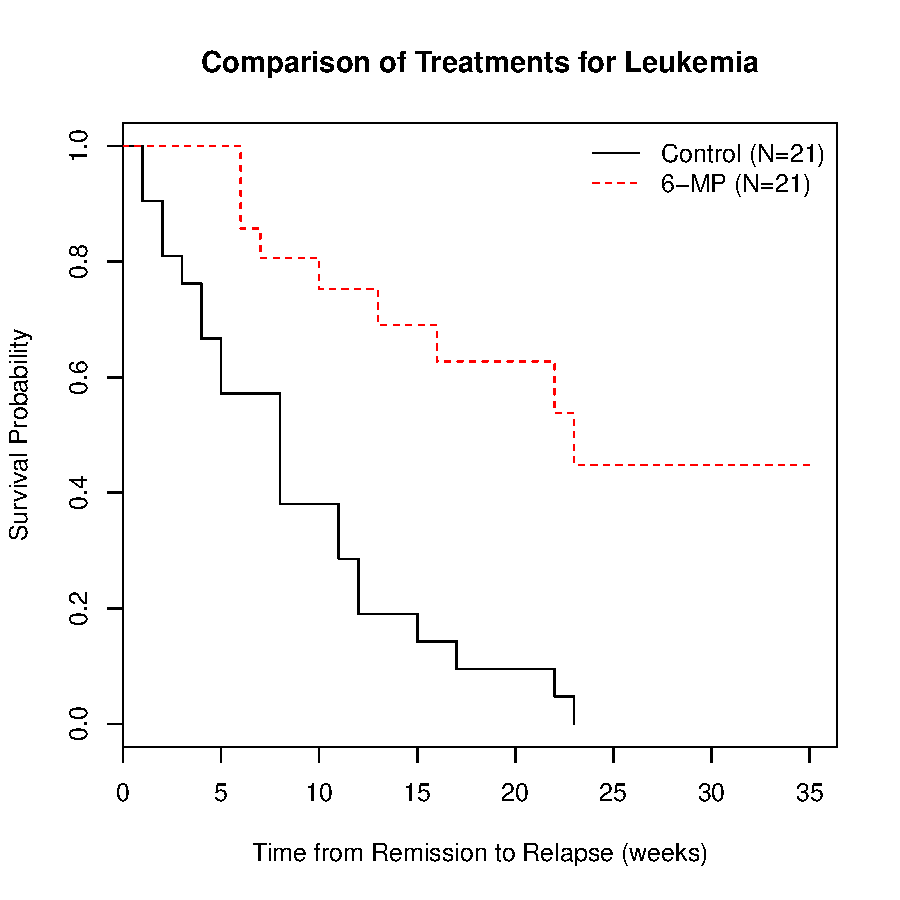
\includegraphics[width=3in]{surv_both.pdf}}
%%%%%%%%%%%%%%%%%%%%%%%%%%%%%%%%%%%%%%%%%%%%%%%%%%%%%%%%%%%%%%%
\end{frame}
\begin{frame}{How can we form a basis for comparison?}
At a specific point in time, we could see whether the confidence intervals for the survival curves overlap.
\\[2ex]
However, the confidence intervals we have been calculating are
{\bf ``pointwise''}  $\Rightarrow$ they correspond to a confidence
interval for $\hat{S}(t^*)$ at a single point in time, $t^{*}$.
\\[2ex]
In other words, we can't say that the true survival function
$S(t)$ is contained between the pointwise confidence intervals with 95\%
probability.
\\[2ex]
({\bf Aside:} if you're interested, the issue of confidence {\bf bands}
for the estimated survival function are discussed in Section 4.4 of
Klein and Moeschberger)
%%%%%%%%%%%%%%%%%%%%%%%%%%%%%%%%%%%%%%%%%%%%%%%%%%%%%%%%%%%%%%%
\end{frame}
\begin{frame}
Looking at whether the confidence intervals for $\hat{S}(t^{*})$ overlap between the 6MP and placebo groups
would only focus on comparing the two treatment
groups at a single point in time, $t^{*}$.
\\[2ex]
{\bf Should we base our overall comparison of $\hat{S}(t)$ on:}
\small
\begin{itemize}
\item the furthest distance between the two curves?
\item the median survival for each group?
\item the average hazard? (for exponential distributions, this would
be like comparing the mean event times)
\item adding differences between the two survival estimates
over time?
\begin{eqnarray*}
\sum_j \; \left[\hat{S}(t_{jA}) - \hat{S}(t_{jB})\right]
\end{eqnarray*}
\vspace*{-.3in}

\item a weighted sum of differences, where the weights reflect the
number at risk at each time?
\item a rank-based test?  i.e., we could rank all of the event times,
and then see whether the sum of ranks for one group was less than the
other.
\end{itemize}
\normalsize
%%%%%%%%%%%%%%%%%%%%%%%%%%%%%%%%%%%%%%%%%%%%%%%%%%%%%%%%%%%%%%%
\end{frame}
\subsection{Nonparametric comparisons of groups}
\begin{frame}{Nonparametric comparisons of groups}

All of these are pretty reasonable options, and we'll see that
there have been several proposals for how to compare the survival
of two groups.  For the moment, we are sticking to nonparametric
comparisons.
\\[2ex]
{\bf Why nonparametric?
\begin{itemize}
\item fairly robust
\item efficient relative to parametric tests
\item often simple and intuitive
\end{itemize}}
Before continuing the description of the two-sample comparison, I'm
going to try to put this in a general framework to give a perspective
of where we're heading in this class.
%%%%%%%%%%%%%%%%%%%%%%%%%%%%%%%%%%%%%%%%%%%%%%%%%%%%%%%%%%%%%%%
\end{frame}
\begin{frame}{General Framework for Survival Analysis}

We observe $(X_i, \delta_i, {\bf Z}_i)$ for individual $i$, where
\begin{itemize}
\item $X_i$ is a censored failure time random variable
\item $\delta_i$ is the failure/censoring indicator
\item ${\bf Z}_i$ represents a set of covariates
\end{itemize}

Note that ${\bf Z}_i$ might be a \underline{scalar} (a single covariate, say
treatment or gender) or may be a $(p\times 1)$ vector (representing
several different covariates).
\end{frame}
\begin{frame}{Types of covariates}
These covariates might be:

\begin{itemize}
\item  continuous
\item  discrete
\item  time-varying (more later)
\end{itemize}

If ${\bf Z}_i$ is a \underline{scalar} and is binary, then we are
comparing the survival of two groups, like in the leukemia example.
\\[2ex]
More generally though, it is useful to build a \underline{model} that
characterizes the relationship between survival and all of the covariates
of interest.
%%%%%%%%%%%%%%%%%%%%%%%%%%%%%%%%%%%%%%%%%%%%%%%%%%%%%%%%%%%%%%%
\end{frame}
\begin{frame}{Comparing two survival distributions}
We'll proceed as follows:
\begin{itemize}
\item  Two group comparisons
\item  Multigroup and stratified comparisons - stratified logrank
\item  Failure time regression models
\begin{itemize}
\item Cox proportional hazards model
\item Accelerated failure time model
\end{itemize}
\end{itemize}
%%%%%%%%%%%%%%%%%%%%%%%%%%%%%%%%%%%%%%%%%%%%%%%%%%%%%%%%%%%%%%%
\end{frame}
\section{Two-sample tests}
\begin{frame}{Two sample tests}

\begin{itemize}
\item Mantel-Haenszel logrank test
\item Peto \& Peto's version of the logrank test
\item Gehan's Generalized Wilcoxon
\item Peto \& Peto's and Prentice's generalized Wilcoxon
\item Tarone-Ware and Fleming-Harrington classes
\item Cox's F-test (non-parametric version)
\end{itemize}

\end{frame} \begin{frame}{References:}
\begin{tabular}{ll}
Collett & Section 2.5\\
Klein \& Moeschberger~~~~ & Section 7.3\\
Kleinbaum &  Chapter 2\\
Lee & Chapter 5\\
\end{tabular}
%%%%%%%%%%%%%%%%%%%%%%%%%%%%%%%%%%%%%%%%%%%%%%%%%%%%%%%%%%%%%%%
\end{frame}
\subsection{The Mantel-Haenszel Logrank test}
\begin{frame}{The Mantel-Haenszel Logrank test}

The logrank test is the most well known and widely used.
\\[2ex]
It also has an intuitive appeal, building on standard
methods for binary data.  (Later we will see that it
can also be obtained as the score test from a partial
likelihood from the Cox Proportional Hazards model.)
\\[2ex]
First consider the following ($2 \times 2$) table classifying those
with and without the event of interest in a two group setting:
\begin{center}
\begin{tabular}{cccc}
\hline \hline
& \multicolumn{2}{c}{Event} & \\ \cline{2-3}
\multicolumn{1}{c}{Group } & ~~~~Yes~~~~ & ~~~~No~~~~ & ~~~Total~~~\\ \hline
0 & $d_0$ & $n_0 - d_0$ & $n_0$  \\
1 & $d_1$ & $n_1 - d_1$ & $n_1$ \\
\hline
Total &  $d  $ & $n   - d  $ & $n  $  \\ \hline \hline
\end{tabular}
\end{center}
%%%%%%%%%%%%%%%%%%%%%%%%%%%%%%%%%%%%%%%%%%%%%%%%%%%%%%%%%%%%%%%
\end{frame}
\begin{frame}{The M-H test (con'd)}

If the margins of this table are considered fixed, then $d_0$
follows a {\em hypergeometric} distribution.  Under the null hypothesis of no association between
the event and group, it follows that
\begin{eqnarray*}
E(d_0) & = & \frac{n_0 d}{n}\\[2ex]
Var(d_0) & = & \frac{n_0 \, n_1 \, d(n-d)}{n^2 (n-1)}
\end{eqnarray*}
Therefore, under $H_0$:\\
\begin{eqnarray*}
\chi^2_{MH} & = & \frac{\left[d_0-n_0 \, d/n\right]^2}{\frac{n_0 \, n_1 \, d(n-d)}
{n^2 (n-1)}} \sim \chi^2_1
\end{eqnarray*}
\end{frame}
\begin{frame}
This is the Mantel-Haenszel statistic and is approximately
equivalent to the Pearson $\chi^2$ test for equality of the two
groups given by:
\begin{eqnarray*}
\chi^2_p & = & \sum \frac{(o-e)^2}{e}
\end{eqnarray*}

Note:  recall that the Pearson $\chi^2$ test was derived for the case where
only the row margins were fixed, and thus the variance above was replaced by:
\begin{eqnarray*}
Var(d_0) & = & \frac{n_0 \, n_1 \, d(n-d)}{n^3}
\end{eqnarray*}
%%%%%%%%%%%%%%%%%%%%%%%%%%%%%%%%%%%%%%%%%%%%%%%%%%%%%%%%%%%%%%%
\end{frame}
\begin{frame}{ Toxicity in a clinical trial with two treatments}

\begin{center}
\begin{tabular}{cccc}
\hline \hline
& \multicolumn{2}{c}{Toxicity}   \\ \cline{2-3}
\multicolumn{1}{c}{Group } & ~~~Yes~~~ & ~~~No~~~ & ~~~Total~~~ \\ \hline
0 &  ~8    & 42  &  ~50       \\
1 &  ~2   &  48 &   ~50        \\
\hline
Total & 10 & 90 &  100        \\ \hline \hline
\end{tabular}
\end{center}

\begin{eqnarray*}
\chi_p^2 & = & 4.00 ~~~~ (p=0.046)\\[3ex]
\chi_{MH}^2 & = & 3.96 ~~~~ (p=0.047)
\end{eqnarray*}
%%%%%%%%%%%%%%%%%%%%%%%%%%%%%%%%%%%%%%%%%%%%%%%%%%%%%%%%%%%%%%%
\end{frame}
\begin{frame}{Generalization of the M-H test}

Now suppose we have $K$ (2$\times 2$) tables, all independent, and we
want to test for a common group effect. The Cochran-Mantel-Haenszel
test for a common odds ratio not equal to 1 can be written as:
\\[2ex]
\[  \chi^2_{CMH} =   \frac{[\sum_{j=1}^K (d_{0j} - n_{0j}*d_j/n_j)]^2}
        {\sum_{j=1}^K n_{1j} n_{0j} d_j (n_j-d_j)/[n_j^2(n_j-1)]}  \]
\\[2ex]
where the subscript $j$ refers to the $j$-th table:

\begin{center}
\begin{tabular}{cccc}
\hline \hline
& \multicolumn{2}{c}{Event} & \\ \cline{2-3}
\multicolumn{1}{c}{Group } & ~~~Yes~~~ & ~~~No~~~ & ~~~Total~~~\\ \hline
0 & $d_{0j}$ & $n_{0j} - d_{0j}$ & $n_{0j}$  \\
1 & $d_{1j}$ & $n_{1j} - d_{1j}$ & $n_{1j}$ \\
\hline
Total &  $d_j  $ & $n_j - d_j  $ & $n_j  $  \\ \hline \hline
\end{tabular}
\end{center}
%\\[2ex]
This statistic is distributed approximately as $\chi^2_1$.
%%%%%%%%%%%%%%%%%%%%%%%%%%%%%%%%%%%%%%%%%%%%%%%%%%%%%%%%%%%%%%%
\end{frame}
\begin{frame}{ How does this apply in survival analysis?}

Suppose we observe

\begin{tabular}{ll}
{\bf Group 1:} &  $(X_{11},\delta_{11}) \dots (X_{1n_1},\delta_{1n_1})$\\[2ex]
{\bf Group 0:} &  $(X_{01},\delta_{01}) \dots (X_{0n_0},\delta_{0n_0})$\\[2ex]
\end{tabular}

We could just count the numbers of failures:
~~eg., $d_1=\sum_{j=1}^K \delta_{1j}$
\end{frame}
\begin{frame}{Example: Leukemia data}
Just counting up the number of remissions in each treatment group.
\begin{center}
\begin{tabular}{cccc}
\hline \hline
& \multicolumn{2}{c}{Fail} &  \\ \cline{2-3}
\multicolumn{1}{c}{Group } & ~~~Yes~~~ & ~~~No~~~ &  ~~~Total~~~  \\ \hline
0 &  21  &   ~0  & 21        \\
1 &  ~9   &  12  & 21        \\
\hline
Total & 30  & 12 & 42    \\ \hline \hline
\end{tabular}
\end{center}
\begin{eqnarray*}
\chi^2_p & = & 16.8 ~~~~ (p=0.001)\\
\chi^2_{MH} & = & 16.4 ~~~~ (p=0.001)
\end{eqnarray*}
But, this doesn't account for the time at risk. Conceptually, we would like to compare the KM survival curves.
Let's put the components side-by-side and compare.
%%%%%%%%%%%%%%%%%%%%%%%%%%%%%%%%%%%%%%%%%%%%%%%%%%%%%%%%%%%%%%%
\end{frame}
\begin{frame}{Cox \& Oakes Table 1.1 Leukemia example}
\scriptsize
\vspace*{-.1in}
\begin{center}
\begin{tabular}{clll|lll}
%\hline
Ordered     & \multicolumn{3}{c}{Group 0} &  \multicolumn{3}{c}{Group 1}  \\ \cline{2-7}
Death Times & $~d_j~$ & $~c_j~$ & $~r_j~$  &  $~d_j~$ & $~c_j~$ & $~r_j~$ \\\hline
  1         &  2      &   0     &  21      &    0    &    0    &   21 \\
  2         &  2      &   0     &  19      &    0    &    0    &   21 \\
  3         &  1      &   0     &  17      &    0    &    0    &   21 \\
  4         &  2      &   0     &  16      &    0    &    0    &   21 \\
  5         &  2      &   0     &  14      &    0    &    0    &   21 \\
  6         &  0      &   0     &  12      &    3    &    1    &   21 \\
  7         &  0      &   0     &  12      &    1    &    0    &   17 \\
  8         &  4      &   0     &  12      &    0    &    0    &   16 \\
  9         &  0      &   0     &  ~8      &    0    &    1    &   16 \\
 10         &  0      &   0     &  ~8      &    1    &    1    &   15 \\
 11         &  2      &   0     &  ~8      &    0    &    1    &   13 \\
 12         &  2      &   0     &  ~6      &    0    &    0    &   12 \\
 13         &  0      &   0     &  ~4      &    1    &    0    &   12 \\
 15         &  1      &   0     &  ~4      &    0    &    0    &   11 \\
 16         &  0      &   0     &  ~3      &    1    &    0    &   11 \\
 17         &  1      &   0     &  ~3      &    0    &    1    &   10 \\
 19         &  0      &   0     &  ~2      &    0    &    1    &   ~9 \\
 20         &  0      &   0     &  ~2      &    0    &    1    &   ~8 \\
 22         &  1      &   0     &  ~2      &    1    &    0    &   ~7 \\
 23         &  1      &   0     &  ~1      &    1    &    0    &   ~6 \\
 25         &  0      &   0     &  ~0      &    0    &    1    &   ~5 \\ \hline
\end{tabular}
\end{center}
\vspace*{-.05in}
\normalsize
We wrote down the number at risk for Group 1 for times 1-5 even though there were no events or censorings at those times.
%%%%%%%%%%%%%%%%%%%%%%%%%%%%%%%%%%%%%%%%%%%%%%%%%%%%%%%%%%%%%%%
\end{frame}
\subsection{Formal definition of the logrank test}
\begin{frame}{ Logrank Test: Formal Definition}

The logrank test is obtained by constructing a ($2 \times 2$) table
at each distinct death time, and comparing the death rates between
the two groups, conditional on the number at risk in the groups.
The tables are then combined using the Cochran-Mantel-Haenszel test.
\\[2ex]
Note: The logrank is sometimes called the Cox-Mantel test.
\\[2ex]
Let $t_1,...,t_K$ represent the $K$ ordered, distinct death times.
\end{frame}
\begin{frame}
At the $j$-th death time, we have the following table:

\begin{center}
\begin{tabular}{cccc}
\hline \hline
& \multicolumn{2}{c}{Die/Fail} & \\ \cline{2-3}
\multicolumn{1}{c}{Group } & ~~~Yes~~~ & ~~~No~~~ & ~~Total~~\\ \hline
0 & $d_{0j}$ & $r_{0j} - d_{0j}$ & $r_{0j}$ \\[2ex]
1 & $d_{1j}$ & $r_{1j} - d_{1j}$ & $r_{1j}$ \\[2ex]
\hline
Total &  $d_j$ & $r_j - d_j$ & $r_j$  \\ \hline \hline
\end{tabular}
\end{center}

where $d_{0j}$ and $d_{1j}$ are the number of deaths in
group 0 and 1, respectively at the $j$-th death time, and
$r_{0j}$ and $r_{1j}$ are the number at risk at that time,
in groups 0 and 1.
%%%%%%%%%%%%%%%%%%%%%%%%%%%%%%%%%%%%%%%%%%%%%%%%%%%%%%%%%%%%%%%
\end{frame}
\begin{frame}
The logrank test is:
\begin{eqnarray*}
\chi^2_{logrank} & = &
\frac{[\sum_{j=1}^K (d_{0j} - r_{0j}*d_j/r_j)]^2}
{\sum_{j=1}^K  \frac{r_{1j} r_{0j} d_j (r_j-d_j)}{[r_j^2(r_j-1)]}}
\end{eqnarray*}
Assuming the tables are all independent, then this statistic
will have an approximate $\chi^2$ distribution with 1 df.
\\[2ex]
{\bf Based on the motivation for the logrank test, which of
the survival-related quantities are we comparing at each
time point?}
\begin{itemize}
\item $\sum_{j=1}^K w_j \left[\hat{S}_1(t_j) - \hat{S}_2(t_j)\right]$ ~~ {\bf ?}
\item $\sum_{j=1}^K w_j \left[\hat\lambda_1(t_j) - \hat\lambda_2(t_j)\right]$ ~~ {\bf ?}
\item $\sum_{j=1}^K w_j \left[\hat\Lambda_1(t_j) - \hat\Lambda_2(t_j)\right]$ ~~ {\bf ?}
\end{itemize}
%%%%%%%%%%%%%%%%%%%%%%%%%%%%%%%%%%%%%%%%%%%%%%%%%%%%%%%%%%%%%%%
\end{frame}
\begin{frame}[fragile]{Example: First several tables of leukemia data}

\scriptsize
\begin{verbatim}
CMH analysis of leukemia data

TABLE 1 OF TRTMT BY REMISS                     TABLE 3 OF TRTMT BY REMISS
CONTROLLING FOR FAILTIME=1                     CONTROLLING FOR FAILTIME=3

TRTMT     REMISS                               TRTMT     REMISS

Frequency|                                     Frequency|
Expected |       0|       1|  Total            Expected |       0|       1|  Total
---------+--------+--------+                   ---------+--------+--------+
       0 |     19 |      2 |     21                   0 |     16 |      1 |     17
         |     20 |      1 |                            | 16.553 | 0.4474 |
---------+--------+--------+                   ---------+--------+--------+
       1 |     21 |      0 |     21                   1 |     21 |      0 |     21
         |     20 |      1 |                            | 20.447 | 0.5526 |
---------+--------+--------+                   ---------+--------+--------+
Total          40        2       42            Total          37        1       38
\end{verbatim}
\end{frame}

\begin{frame}[fragile]{}

\scriptsize
\begin{verbatim}
TABLE 2 OF TRTMT BY REMISS                     TABLE 4 OF TRTMT BY REMISS
CONTROLLING FOR FAILTIME=2                     CONTROLLING FOR FAILTIME=4

TRTMT     REMISS                               TRTMT     REMISS

Frequency|                                     Frequency|
Expected |       0|       1|  Total            Expected |       0|       1|  Total
---------+--------+--------+                   ---------+--------+--------+
       0 |     17 |      2 |     19                   0 |     14 |      2 |     16
         |  18.05 |   0.95 |                            | 15.135 | 0.8649 |
---------+--------+--------+                   ---------+--------+--------+
       1 |     21 |      0 |     21                   1 |     21 |      0 |     21
         |  19.95 |   1.05 |                            | 19.865 | 1.1351 |
---------+--------+--------+                   ---------+--------+--------+
Total          38        2       40            Total          35        2       37
\end{verbatim}
%%%%%%%%%%%%%%%%%%%%%%%%%%%%%%%%%%%%%%%%%%%%%%%%%%%%%%%%%%%%%%%
\end{frame}

\begin{frame}[fragile]{CMH statistic = logrank statistic}

\scriptsize
\begin{verbatim}
              SUMMARY STATISTICS FOR TRTMT BY REMISS
                    CONTROLLING FOR FAILTIME


 Cochran-Mantel-Haenszel Statistics (Based on Table Scores)

Statistic   Alternative Hypothesis    DF       Value      Prob
-----------------------------------------------------------------
    1        Nonzero Correlation        1      16.793     0.001
    2        Row Mean Scores Differ     1      16.793     0.001
    3        General Association        1      16.793     0.001 <===LOGRANK
                                                                    TEST
\end{verbatim}

\normalsize
Note: Although CMH works to get the correct logrank test, it would
require inputting the $d_j$ and $r_j$ at each time of death
for each treatment group.  There's an easier way to get the
test statistic, which I'll show you shortly.
%%%%%%%%%%%%%%%%%%%%%%%%%%%%%%%%%%%%%%%%%%%%%%%%%%%%%%%%%%%%%%%
\end{frame}

\begin{frame}{Calculating logrank statistic by hand: Leukemia Example:}
\small
\begin{center}
\begin{tabular}{ccccccccc}
\hline
Ordered     & \multicolumn{2}{c}{Group 0} &  \multicolumn{2}{c}{Combined}  \\
\cline{2-3} \cline{4-5}
Death Times & $~d_{0j}~$ & $~r_{0j}~$  & $~d_{j}~$ & $~r_{j}~$ &
     ~$e_j$~ & ~~$o_j-e_j$~~ & ~~$v_j$~~ \\ \hline
  1   &  2    &  21   &    2    &   42  & 1.00 & 1.00 & 0.488\\
  2   &  2    &  19   &    2    &   40  & 0.95 & 1.05 \\
  3   &  1    &  17   &    1    &   38  & 0.45 & 0.55 \\
  4   &  2    &  16   &    2    &   37  & 0.86 & 1.14 \\
  5   &  2    &  14   &    2    &   35  & \\
  6   &  0    &  12   &    3    &   33  & \\
  7   &  0    &  12   &    1    &   29  & \\
  8   &  4    &  12   &    4    &   28  & \\
 10   &  0    &  ~8   &    1    &   23  & \\
 11   &  2    &  ~8   &    2    &   21  & \\
 12   &  2    &  ~6   &    2    &   18  & \\
 13   &  0    &  ~4   &    1    &   16  & \\
 15   &  1    &  ~4   &    1    &   15  & \\
 16   &  0    &  ~3   &    1    &   14  & \\
 17   &  1    &  ~3   &    1    &   13  & \\
 22   &  1    &  ~2   &    2    &   ~9  & \\
 23   &  1    &  ~1   &    2    &   ~7  & \\ \hline
Sum   &       &       &         &       &    & 10.251 & 6.257 \\
\end{tabular}
\end{center}
\normalsize
\end{frame}

\begin{frame}
In the previous table
\\[2ex]
$o_j = d_{0j}$\\[1ex]
$e_j = d_j r_{0j}/r_j$ \\[1ex]
$v_j = r_{1j} r_{0j} d_j (r_j-d_j)/[r_j^2(r_j-1)]$
\begin{eqnarray*}
\chi^2_{logrank} & = & \frac{(10.251)^2}{6.257} ~=~ 16.793
\end{eqnarray*}
%%%%%%%%%%%%%%%%%%%%%%%%%%%%%%%%%%%%%%%%%%%%%%%%%%%%%%%%%%%%%%%
\end{frame}
\begin{frame}{ Notes about logrank test:}
\begin{itemize}
\item The logrank statistic depends on ranks of event times only
\item If there are no tied deaths, then the logrank has the form:
\[    \frac{[\sum_{j=1}^K (d_{0j} - \frac{r_{0j}}{r_j})]^2}
        {\sum_{j=1}^K r_{1j}r_{0j}/r_j^2}  \]
\item  Numerator can be interpreted as $\sum (o-e)$ where
``o'' is the observed number of deaths in group 0, and
``e'' is the expected number, given the risk set.  The expected
number equals \#deaths $\times$ proportion in group 0
at risk.
\item  The ($o-e$) terms in the numerator  can be written as
\[   \frac{r_{0j}r_{1j}}{r_j}(\hat\lambda_{1j} - \hat\lambda_{0j} ) \]
\end{itemize}
\end{frame}
\begin{frame}{Notes about the logrank test (cont'd)}
\begin{itemize}
\item  It does not matter which group you choose to sum over.
 To see this, note that if we summed up (o-e) over the death
times for the 6MP group we would get -10.251, and the sum of the
variances is the same.  So when we square the numerator, the test
statistic is the same.
\end{itemize}
%%%%%%%%%%%%%%%%%%%%%%%%%%%%%%%%%%%%%%%%%%%%%%%%%%%%%%%%%%%%%%%
Analogous to the CMH test for a series of tables at
different levels of a confounder, the logrank test is most powerful when
``odds ratios'' are constant over time intervals.
\\[2ex]
That is, it is most powerful for {\bf proportional hazards}.
\end{frame}
\begin{frame}{Checking the assumption of proportional hazards:}
We check the assumption of proportional hazards as follows:
\begin{itemize}
\item check to see if the estimated survival curves cross - if they
do, then this is evidence that the hazards are \underline{not} proportional
\item more formal test: {\bf any ideas?}
\end{itemize}
{\bf What should be done if the hazards are \underline{not }\\
proportional?}

\begin{itemize}
\item If the difference between hazards has a consistent sign, the logrank
test usually does well.
\item Other tests are available that are more powerful against different
alternatives.
\end{itemize}
%%%%%%%%%%%%%%%%%%%%%%%%%%%%%%%%%%%%%%%%%%%%%%%%%%%%%%%%%%%%%%%
\end{frame}
\subsection{Computer implementation}
\begin{frame}[fragile]{Getting the logrank statistic using R}
Listing of the leukemia survival.

\scriptsize
\begin{verbatim}

                trt=Control
 time n.risk n.event survival std.err lower 95% CI upper 95% CI
    1     21       2   0.9048  0.0641      0.78754        1.000
    2     19       2   0.8095  0.0857      0.65785        0.996
    3     17       1   0.7619  0.0929      0.59988        0.968
    4     16       2   0.6667  0.1029      0.49268        0.902
    5     14       2   0.5714  0.1080      0.39455        0.828
    8     12       4   0.3810  0.1060      0.22085        0.657
   11      8       2   0.2857  0.0986      0.14529        0.562
   12      6       2   0.1905  0.0857      0.07887        0.460
   15      4       1   0.1429  0.0764      0.05011        0.407
   17      3       1   0.0952  0.0641      0.02549        0.356
   22      2       1   0.0476  0.0465      0.00703        0.322
   23      1       1   0.0000     NaN           NA           NA

                trt=6-MP
 time n.risk n.event survival std.err lower 95% CI upper 95% CI
    6     21       3    0.857  0.0764        0.720        1.000
    7     17       1    0.807  0.0869        0.653        0.996
   10     15       1    0.753  0.0963        0.586        0.968
   13     12       1    0.690  0.1068        0.510        0.935
   16     11       1    0.627  0.1141        0.439        0.896
   22      7       1    0.538  0.1282        0.337        0.858
   23      6       1    0.448  0.1346        0.249        0.807
\end{verbatim}
\end{frame}

\begin{frame}[fragile]{Calculating the Logrank test with R}
\begin{verbatim}

             N Observed Expected (O-E)^2/E (O-E)^2/V
trt=Control 21       21     10.7      9.77      16.8
trt=6-MP    21        9     19.3      5.46      16.8

 Chisq= 16.8  on 1 degrees of freedom, p= 4.17e-05
\end{verbatim}
%%%%%%%%%%%%%%%%%%%%%%%%%%%%%%%%%%%%%%%%%%%%%%%%%%%%%%%%%%%%%%%
\end{frame}

\section{Generalization of the logrank test}
\subsection{Linear rank tests}

\begin{frame}{Generalization of logrank test: Linear rank tests}

The logrank and other tests can be derived by assigning scores to the
ranks of the death times, and are members of a general class
of {\bf linear rank tests} (for more detail, see Lee, ch 5)

First, define
\begin{eqnarray*}
\hat\Lambda(t) = \sum_{j: t_j <t} \frac{d_j}{r_j}
\end{eqnarray*}
where $d_j$ and $r_j$ are the number of deaths and the
number at risk, respectively at the $j$-th ordered death
time.
\end{frame}

\begin{frame}{The Peto \& Peto approach}
Then assign these scores (suggested by Peto and Peto):
\begin{center}
\begin{tabular}{ll}
\hline \hline
{\sc Event} & {\sc Score} \\ \hline
Death at $t_j$ & $w_j=1 - \hat\Lambda(t_j)$\\[1ex]
Censoring at $t_j$~~~~~ & $w_j= - \hat\Lambda(t_j)$\\
\hline
\end{tabular}
\end{center}
~\\[2ex]
To calculate the logrank test, simply sum up the scores for group 0.
%%%%%%%%%%%%%%%%%%%%%%%%%%%%%%%%%%%%%%%%%%%%%%%%%%%%%%%%%%%%%%%
\begin{tabular}{lll}
\underline{\bf Example}~~ & Group 0: & 15, 18, 19, 19, 20 \\[1ex]
                          & Group 1: & 16$+$, 18$+$, 20$+$, 23, 24$+$
\end{tabular}

\end{frame}

\begin{frame}{Calculation of logrank as a linear rank statistic}
\begin{center}
\begin{tabular}{cccccc}
\hline
Ordered Data & Group & ~~$d_j$~~ & ~~$r_j$~~ &  $\hat\Lambda(t_j)$ & score $w_j$  \\
\hline
$15~$     &   0   &     1   &   10  &  0.100   & ~0.900 \\
$16^+$    &   1   &     0   &   ~9  &  0.100   & -0.100 \\
$18~$     &   0   &     1   &   ~8  &  0.225   & ~0.775 \\
$18^+$    &   1   &     0   &   ~7  &  0.225   & -0.225 \\
$19~$     &   0   &     2   &   ~6  &  0.558   & ~0.442 \\
$20~$     &   0   &     1   &   ~4  &  0.808   & ~0.192 \\
$20^+$    &   1   &     0   &   ~3  &  0.808   & -0.808 \\
$23~$     &   1   &     1   &   ~2  &  1.308   & -0.308 \\
$24^+$    &   1   &     0   &   ~1  &  1.308   & -1.308 \\ \hline
\end{tabular}
\end{center}

The logrank statistic $S$ is sum of scores for group 0:
\[ S = 0.900 + 0.775 + 0.442 + 0.442 + 0.192=2.75\]
\end{frame}
\begin{frame}{Variance of the linear rank test}
The variance is:
\[ Var(S) = \frac{n_0 n_1 \sum_{j=1}^{n} w_j^2 }{n(n-1)} \]
\\[2ex]
In this case,  $Var(S)= 1.210$, so
\begin{eqnarray*}
Z = \frac{2.75}{\sqrt{1.210}} = 2.50
& \Longrightarrow & \chi^2_{logrank} = (2.50)^2 = 6.25
\end{eqnarray*}
%%%%%%%%%%%%%%%%%%%%%%%%%%%%%%%%%%%%%%%%%%%%%%%%%%%%%%%%%%%%%%%
\end{frame}

\begin{frame}{Why is this form of the logrank equivalent?}

The logrank statistic S is equivalent to $\sum (o-e)$ over
the distinct death times, where ``$o$'' is the observed number of
deaths in group 0, and ``$e$'' is the expected number, given
the risk sets.
\begin{center}
\begin{tabular}{ll}
{\bf At deaths:} & weights are $1-\hat\Lambda$\\
{\bf At censorings:}~~~~ & weights are $-\hat\Lambda$
\end{tabular}
\end{center}

So we are summing up ``1's'' for deaths (to get $d_{0j}$), and subtracting
$-\hat\Lambda$ at both deaths and censorings.  This amounts
to subtracting $d_j/r_j$ at each death or censoring
time in group 0, at or after the $j$-th death.  Since there are
a total of $r_{0j}$ of these, we get $e = r_{0j} * d_j/r_j$.

\end{frame}
\begin{frame}{Why is it called the {\bf logrank} test?}

Since $S(t) = \exp(-\Lambda(t))$, an alternative estimator of $S(t)$ is:
\[  \hat{S}(t) = \exp\left (-\hat\Lambda(t)\right ) = \exp\left ( - \sum_{j: t_j<t} \frac{d_j}{r_j}\right )\]

So,  we can think of $\hat\Lambda(t)=-\log(\hat{S}(t))$ as yielding the
``log-survival'' scores used to calculate the statistic.
%%%%%%%%%%%%%%%%%%%%%%%%%%%%%%%%%%%%%%%%%%%%%%%%%%%%%%%%%%%%%%%
\end{frame}

%\subsection{Comparison between the CMH and Linear-rank logrank tests}
\begin{frame}{Comparing the CMH-type Logrank and ``Linear Rank'' logrank}

\underline{\bf A. CMH-type Logrank:}\\[1ex]
We motivated the logrank test through the CMH statistic for
testing $H_o: OR=1$ over $K$ tables, where $K$ is the number
of distinct death times.  This turned out to be what we get
when we use the logrank (default) option in Stata. (or the
``{\sc strata}'' statement in SAS)
~\\[2ex]
\underline{\bf B. Linear Rank logrank:}\\[1ex]
The linear rank version of the logrank test is based
on adding up ``scores'' for one of the two treatment groups.
The particular scores that gave us the same logrank statistic were
based on the Nelson-Aalen estimator, i.e.,
$\hat\Lambda = \sum \hat\lambda(t_j)$.
This is what you get when you use the ``{\sc test}''
statement in SAS.
%%%%%%%%%%%%%%%%%%%%%%%%%%%%%%%%%%%%%%%%%%%%%%%%%%%%%%%%%%%%%%%
\end{frame}

\begin{frame}
If there are no tied event times, then the two versions of the
test will yield identical results.  The more ties we have, the
more it matters which version we use.

The numerators of the two types
of logrank tests will always be equivalent, but the denominators
depend on the way ties are handled:

{\bf CMH-type variance:}
\begin{eqnarray*}
var & = & \sum \frac{r_{1j} r_{0j} d_j (r_j-d_j)}{r_j^2(r_j-1)}\\
    & = & \sum \frac{r_{1j} r_{0j}}{r_j (r_j-1)} \; \frac{d_j (r_j-d_j)}{r_j}\\
\end{eqnarray*}

{\bf Linear rank type variance:}
\begin{eqnarray*}
var & = & \frac{n_0 n_1 \sum_{j=1}^{n} w_j^2 }{n(n-1)}
\end{eqnarray*}
%%%%%%%%%%%%%%%%%%%%%%%%%%%%%%%%%%%%%%%%%%%%%%%%%%%%%%%%%%%%%%%
\end{frame}

%\subsection{Gehan's test}
\begin{frame}{Review of the Wilcoxon Test}

First, let's review the Wilcoxon test for uncensored data:\\[1ex]
Denote observations from two samples by:
$$(X_1,X_2, \ldots, X_n) ~~\mbox{and}~~ (Y_1,Y_2,\ldots,Y_m)$$
Order the combined sample and define:
\[Z_{(1)}<Z_{(2)}<\cdots<Z_{(m+n)}\]
\[R_{i1}=\mbox{rank of }X_i\]
\[R_1=\sum_{i=1}^{m+n} R_{i1}\]
\end{frame}
\begin{frame}{Review of the Wilcoxon test (cont'd)}
Reject $H_0$ if $R_1$ is too big or too small, according to
\[\frac{R_1-E(R_1)}{\sqrt{Var(R_1)}}\sim N(0,1)\]

where
\begin{eqnarray*}
E(R_1) & = & \frac{m(m+n+1)}{2}\\[1ex]
Var(R_1) & = & \frac{mn(m+n+1)}{12}
\end{eqnarray*}
%%%%%%%%%%%%%%%%%%%%%%%%%%%%%%%%%%%%%%%%%%%%%%%%%%%%%%%%%%%%%%%
\end{frame}

\begin{frame}{The Mann-Whitney form of the Wilcoxon test}

This is defined as:\\[0.5ex]
\[U(X_i,Y_j)=U_{ij}=\left\{\begin{array}{ccc}
+1 & \mbox{ if } & X_i>Y_j\\
~0 & \mbox{ if } & X_i=Y_j\\
-1 & \mbox{ if } & X_i<Y_j
\end{array} \right.\]
and
\[U=\sum_{i=1}^n \sum_{j=1}^m U_{ij}.\]

~\\[2ex]
There is a simple correspondence between $U$ and $R_1$:
\begin{eqnarray*}
R_1 & = & m(m+n+1)/2+U/2\\[2ex]
\mbox{so}~~~~~~~~ U & = & 2 R_1 - m(m+n+1)\\[3ex]
\end{eqnarray*}
~\\[-2ex]
Therefore, $E(U) =  0$ and $Var(U) = mn(m+n+1)/3$.
%%%%%%%%%%%%%%%%%%%%%%%%%%%%%%%%%%%%%%%%%%%%%%%%%%%%%%%%%%%%%%%
\end{frame}

\begin{frame}{Extending Wilcoxon to censored data}

The Mann-Whitney form leads to a generalization
for censored data.  Define
\[U(X_i,Y_j)=U_{ij}=\left\{\begin{array}{ccl}
+1 & \mbox{ if } & ~~x_i>y_j \mbox{~~or~~} x_i^+\geq y_j\\
~0 & \mbox{ if } & ~~x_i=y_i \mbox{~~or lower value censored}\\
-1 & \mbox{ if } & ~~x_i<y_j \mbox{~~or~~} x_i \leq y_j^+
\end{array} \right. \]

Then define $$W=\sum_{i=1}^{n} \sum_{j=1}^{m} U_{ij}$$
\\[2ex]
Thus, there is a contribution to $W$ for every comparison
where both observations are failures (except for ties), or
where a censored observation is greater than or equal to a failure.
\\[2ex]
Looking at all possible pairs of individuals between the
two treatment groups makes this a nightmare to compute by
hand!
%%%%%%%%%%%%%%%%%%%%%%%%%%%%%%%%%%%%%%%%%%%%%%%%%%%%%%%%%%%%%%%
\end{frame}

\begin{frame}{Gehan's Generalized Wilcoxon test}

Gehan found an easier way to compute the above.  First, pool
the sample of ($n+m$) observations into a single group, then
compare each individual with the remaining $n+m-1$:  For
comparing the $i$-th individual with the $j$-th, define
\[ U_{ij}=\left\{\begin{array}{ccc}
+1 & \mbox{ if } & ~~t_i>t_j \mbox{~~or~~} t_i^+\geq t_j\\
-1 & \mbox{ if } & ~~t_i<t_j \mbox{~~or~~} t_i \leq t_j^+\\
~0 &             & ~~otherwise\\
\end{array} \right. \]
\end{frame}
\begin{frame}{Gehan's statistic}
Then
$$U_i=\sum_{j=1}^{m+n} U_{ij}$$

Thus, for the $i$-th individual, $U_i$ is the number of
observations which are \underline{definitely less} than $t_i$
minus the number of observations that are \underline{definitely
greater} than $t_i$.  We assume censorings occur after deaths,
so that if $t_i=18^+$ and $t_j=18$, then we add 1 to $U_i$.
\\[2ex]
The Gehan statistic is defined as
\begin{eqnarray*}
U & = & \sum_{i=1}^{m+n} U_i \; {\bf 1}_{\{i \mbox{ in group 0}\}}\\[2ex]
  & = & W
\end{eqnarray*}

$U$ has mean 0 and variance
\[var(U) = \frac{mn}{(m+n)(m+n-1)}\sum_{i=1}^{m+n} U_i^2\]
%%%%%%%%%%%%%%%%%%%%%%%%%%%%%%%%%%%%%%%%%%%%%%%%%%%%%%%%%%%%%%%
\end{frame}

\begin{frame}{Example from Lee}
Group 0:~~ 15, 18, 19, 19, 20 ~~ Group 1:~~ 16$+$, 18$+$, 20$+$, 23, 24$+$
\scriptsize
\begin{center}
\begin{tabular}{cccc}
\hline \hline
Time & Group & ~~~$U_i$~~~ & ~~~$U_i^2$~~~ \\ \hline
15~    & 0 & ~-9 & ~81 \\
16$^+$ & 1 & ~~1 & ~~1 \\
18~    & 0 & ~-6 & ~36 \\
18$^+$ & 1 & ~~2 & ~~4 \\
19~    & 0 & ~-2 & ~~4 \\
19~    & 0 & ~-2 & ~~4 \\
20~    & 0 & ~~1 & ~~1 \\
20$^+$ & 1 & ~~5 & ~25 \\
23~    & 1 & ~~4 & ~16 \\
24$^+$ & 1 & ~~6 & ~36 \\ \hline
SUM    &   & -18 & 208 \\ \hline \hline
\end{tabular}
\end{center}
\small
\begin{eqnarray*}
U & = & -18 ~~~~ Var(U) = \frac{(5)(5)(208)}{(10)(9)} = 57.78\\
\mbox{and}~~~ \chi^2 & = & (-18)^2/57.78 = 5.61
\end{eqnarray*}
%%%%%%%%%%%%%%%%%%%%%%%%%%%%%%%%%%%%%%%%%%%%%%%%%%%%%%%%%%%%%%%
\end{frame}
%\subsection{The Peto \& Peto generalized Wilcoxon test}
\begin{frame}{Generalized Wilcoxon} (Peto \& Peto, Prentice)

Assign the following scores:\\
\begin{center}
\begin{tabular}{ll}
~~~~For a death at $t$: &             $\hat{S}(t+) + \hat{S}(t-) -1$\\
~~~~For a censoring at $t$:~~~~~~~  & $\hat{S}(t+) - 1$
\end{tabular}
\end{center}

The test statistic is $\sum(scores)$  for group 0.
\scriptsize
\begin{center}
\begin{tabular}{cccccc}
\hline
Time & Group & ~~$d_j$~~ & ~~$r_j$~~ & ~~$\hat{S}(t+)$~~ & score $w_j$\\ \hline
$15~$     &     0   &   1   &   10      & 0.900 & ~0.900 \\
$16^+$    &     1   &   0   &   ~9  & 0.900 & -0.100 \\
$18~$     &     0   &   1   &   ~8  & 0.788 & ~0.688 \\
$18^+$    &     1   &   0   &   ~7  & 0.788 & -0.212 \\
$19~$     &     0   &   2   &   ~6  & 0.525 & ~0.313 \\
$20~$     &     0   &   1   &   ~4  & 0.394 & -0.081 \\
$20^+$    &     1   &   0   &   ~3  & 0.394 & -0.606 \\
$23~$     &     1   &   1   &   ~2  & 0.197 & -0.409 \\
$24^+$    &     1   &   0   &   ~1  & 0.197 & -0.803 \\ \hline
\end{tabular}
\end{center}
\end{frame}

\begin{frame}
\begin{eqnarray*}
\sum w_j \, {\bf 1}_{\{j \mbox{ in group 0}\}}
& = & 0.900 + 0.688 + 2*(0.313) + (-0.081) \\
& = & 2.13\\[2ex]
Var(S) & = & \frac{n_0 n_1 \sum_{j=1}^{n} w_j^2 }{n(n-1)} ~=~ 0.765\\[1ex]
\mbox{so}~~~~ Z & = & 2.13/0.765 ~=~ 2.433
\end{eqnarray*}
%%%%%%%%%%%%%%%%%%%%%%%%%%%%%%%%%%%%%%%%%%%%%%%%%%%%%%%%%%%%%%%
\end{frame}
\subsection{Computer implementation}
\begin{frame}[fragile]{Obtaining the Wilcoxon test using R}

{ \bf Example: (leukemia data)}
%\scriptsize
\begin{verbatim}
             N Observed Expected (O-E)^2/E (O-E)^2/V
trt=Control 21    14.55     7.68      6.16      14.5
trt=6-MP    21     5.12    12.00      3.94      14.5

 Chisq= 14.5  on 1 degrees of freedom, p= 0.000143
\end{verbatim}
%%%%%%%%%%%%%%%%%%%%%%%%%%%%%%%%%%%%%%%%%%%%%%%%%%%%%%%%%%%%%%%
\end{frame}

\subsection{The Tarone \& Ware class of tests}
\begin{frame}{The Tarone-Ware class of tests}

This general class of tests is like the logrank test, but
adds weights $w_j$.  The logrank test, Wilcoxon test, and
Peto-Prentice Wilcoxon are included as special cases.

\[ \chi^2_{tw} = \frac{[\sum_{j=1}^K w_j (d_{1j} - r_{1j}*d_j/r_j)]^2}
        {\sum_{l=1}^K \frac{w_j^2 r_{1j}r_{0j}d_j(r_j-d_j)}{r_j^2(r_j-1)}}  \]
\end{frame}

\begin{frame}{The Tarone-Ware tests (cont'd)}

\begin{center}
\begin{tabular}{ll}
\hline \hline
{\bf Test} & {\bf Weight $w_j$} \\ \hline
Logrank              &  $w_j = 1$\\[2ex]
Gehan's Wilcoxon     &  $w_j = r_j$\\[2ex]
Peto/Prentice        &  $w_j = n \widehat{S}(t_j)$\\[2ex]
Fleming-Harrington~~~~   &  $w_j=[\hat{S}(t_j)]^\alpha$\\[2ex]
Tarone-Ware          &  $w_j=\sqrt{r_j}$\\
\hline \hline
\end{tabular}
\end{center}

Note:  these weights $w_j$ are not the same as the scores $w_j$
we've been talking about earlier, and they apply to the CMH-type
form of the test statistic rather than $\sum (scores)$ over
a single treatment group.
%%%%%%%%%%%%%%%%%%%%%%%%%%%%%%%%%%%%%%%%%%%%%%%%%%%%%%%%%%%%%%%
\end{frame}

\begin{frame}{Which test should we used?}

\underline{\bf CMH-type or Linear Rank?}\\
If there are not a high proportion of ties, then it doesn't
really matter since:
\begin{itemize}
\item  The two Wilcoxons are similar to each other
\item  The two logrank tests are similar to each other
\end{itemize}
{ Note: personally, I tend to use the CMH-type test, which
you get with the {\sc strata} statement in SAS and the {\sc test}
statement in STATA.}
\end{frame}

\begin{frame}{Logrank or Wilcoxon?}
\begin{itemize}
\item Both tests have the right Type I power for testing the null
hypothesis of equal survival, $H_o: S_1(t)=S_2(t)$

\item The choice of which test may therefore depend on the alternative
hypothesis, which will drive the \underline{power} of the test.
\item The Wilcoxon is sensitive to early differences between survival,
while the logrank is sensitive to later ones.  This can be seen by
the relative weights they assign to the test statistic:
\begin{eqnarray*}
\mbox{LOGRANK} ~~~~ {\rm numerator} & = & \sum_j (o_j - e_j)\\[1ex]
\mbox{WILCOXON} ~~~ {\rm numerator} & = & \sum_j r_j (o_j - e_j)\\
\end{eqnarray*}
\end{itemize}
\end{frame}

\begin{frame}
\begin{itemize}
\item The logrank is most powerful under the assumption of
proportional hazards, which implies an alternative in terms
of the survival functions of $H_a: S_1(t)=[S_2(t)]^{\alpha}$
\item The Wilcoxon has high power when the failure times are
lognormally distributed, with equal variance in both groups but a
different mean.  It will turn out that this is the assumption of
an accelerated failure time model.
\item  Both tests will lack power if the survival curves
(or hazards) ``cross''.  However, that does not necessarily
make them invalid!
\end{itemize}
%%%%%%%%%%%%%%%%%%%%%%%%%%%%%%%%%%%%%%%%%%%%%%%%%%%%%%%%%%%%%%%

\end{frame}
\section{The $P$-sample and stratified  logrank tests}
\subsection{The $P$-sample logrank test}
\begin{frame}{$P$-sample logrank tests}

We have been discussing two sample problems.  In practice,
more complex settings often arise:
\begin{itemize}
\item There are more than two treatments or groups, and the question of
 interest is whether the groups differ from each other.
\item We are interested in a comparison between  two groups, but we
wish to adjust for another factor that may confound  the analysis
\item We want to adjust for lots of covariates.
\end{itemize}

We will first talk about comparing the survival distributions
between more than 2 groups, and then about adjusting for other
covariates.
%%%%%%%%%%%%%%%%%%%%%%%%%%%%%%%%%%%%%%%%%%%%%%%%%%%%%%%%%%%%%%%
\end{frame}
\begin{frame}{The $P$-sample logrank test (cont'd)}

Suppose we observe data from $P$ different groups, and
 the data from group $p$ ($p=1,...,P$) are:
\[ (X_{p1},\delta_{p1}) \dots
(X_{p n_p},\delta_{p n_p}) \]

We now contruct a $(P \times 2)$ table at each of
the $K$ distinct death times, and compare the death rates
between the $P$ groups, conditional on the number at risk.
\end{frame}
\begin{frame}
Let $t_1,....t_K$ represent the $K$ ordered, distinct death
times.\\[2ex]
At the $j$-th death time, we have the following table:

\begin{center}
\begin{tabular}{cccc}
\hline \hline
& \multicolumn{2}{c}{Die/Fail} & \\ \cline{2-3}
\multicolumn{1}{c}{Group } & ~~~Yes~~~ & ~~~No~~~ & ~~~Total~~~\\ \hline
1 &  $d_{1j}$  & $r_{1l} - d_{1j}$ & $r_{1j}$ \\[2ex]
. &    .       &     .             &       .    \\[2ex]
P & $d_{Pj}$   & $r_{Pj} - d_{Pj}$ & $r_{Pj}$  \\ \hline
Total &  $d_j  $ & $r_j - d_j  $ & $r_j  $  \\ \hline \hline
\end{tabular}
\end{center}

where $d_{pj}$ is  the number of deaths in group $p$ at the $j$-th death time, and
$r_{pj}$ is the number at risk at that time.
\\[2ex]
The tables are then combined using the CMH approach.
%%%%%%%%%%%%%%%%%%%%%%%%%%%%%%%%%%%%%%%%%%%%%%%%%%%%%%%%%%%%%%%

If we were just focusing on this one table, then a $\chi^2_{(P-1)}$
test statistic could be constructed through a comparison of ``o''s and
``e''s, like before.
\end{frame}

\begin{frame}[fragile]{Example: Toxicity in a clinical trial with 3 treatments}
Consider a clinical trial with three treatments.

\scriptsize
\begin{verbatim}
TABLE OF GROUP BY TOXICITY

GROUP     TOXICITY

Frequency|
Row Pct  |no      |yes     |  Total
---------+--------+--------+
       1 |     42 |      8 |     50
         |  84.00 |  16.00 |
---------+--------+--------+
       2 |     48 |      2 |     50
         |  96.00 |   4.00 |
---------+--------+--------+
       3 |     38 |     12 |     50
         |  76.00 |  24.00 |
---------+--------+--------+
Total         128       22      150
\end{verbatim}
\end{frame}

\begin{frame}[fragile]

\scriptsize
\begin{verbatim}
STATISTICS FOR TABLE OF GROUP BY TOXICITY

Statistic                     DF     Value        Prob
------------------------------------------------------
Chi-Square                     2     8.097       0.017
Likelihood Ratio Chi-Square    2     9.196       0.010
Mantel-Haenszel Chi-Square     1     1.270       0.260

  Cochran-Mantel-Haenszel Statistics (Based on Table Scores)

Statistic   Alternative Hypothesis    DF    Value     Prob
----------------------------------------------------------
   1        Nonzero Correlation        1    1.270    0.260
   2        Row Mean Scores Differ     2    8.043    0.018
   3        General Association        2    8.043    0.018
\end{verbatim}
%%%%%%%%%%%%%%%%%%%%%%%%%%%%%%%%%%%%%%%%%%%%%%%%%%%%%%%%%%%%%%%
\end{frame}

\begin{frame}{Formal Calculations}

Let ${\bf O}_j = (d_{1j},...d_{(P-1)j})^T$ be a vector
of the observed number of failures in groups 1 to $(P-1)$,
respectively, at the $j$-th death time. \\[2ex]
Given the risk sets $r_{1j}$, ... $r_{Pj}$, and the fact that there are
$d_j$ deaths, then ${\bf O}_j$ has a distribution like a
multivariate version of the hypergeometric.  \\[2ex]

${\bf O}_j$ has mean:

\[   {\bf E}_j =\left (\frac{d_{j}\, r_{1j}}{r_j},~...~,
\frac{d_{j} \, r_{(P-1)j}}{r_j}\right )^T \]
\end{frame}

\begin{frame}{Variance covariance matrix}
and variance covariance matrix:
  \[   {\bf V}_j = \left( \begin{array}{cccc}
                          v_{11j} & v_{12j} & ... & v_{1(P-1)j} \\
                                  & v_{22j} & ... & v_{2(P-1)j} \\
                              ... &         & ... & ... \\
                                  &         &     & v_{(P-1)(P-1)j} \\
                    \end{array} \right)  \]

where the $\ell$-th diagonal element is:
\[     v_{\ell\ell j} = r_{\ell j}(r_j-r_{\ell j})
d_j(r_j-d_j)/[r_j^2(r_j-1)]  \]

and the $\ell m$-th off-diagonal element is:
\[     v_{\ell m j} = r_{\ell j}r_{mj}d_j(r_j-d_j)/[r_j^2(r_j-1)]  \]
%%%%%%%%%%%%%%%%%%%%%%%%%%%%%%%%%%%%%%%%%%%%%%%%%%%%%%%%%%%%%%%
The resulting $\chi^2$ test for a single $(P \times 1)$ table would
have (P-1) degrees and is constructed as follows:
\[   ( {\bf O}_j - {\bf E}_j)^T \; {\bf V}^{-1}_j \; ( {\bf O}_j - {\bf E}_j)
\]

\end{frame}

\begin{frame}{Generalizing to $K$ tables}

Analogous to what we did for the two sample logrank, we replace the
$ {\bf O}_j$, ${\bf E}_j$ and ${\bf V}_j$ with the sums over the
$K$ distinct death times. \\[2ex]
That is, let
 $ {\bf O} = \sum_{j=1}^{k}  {\bf O}_j$,
 $ {\bf E} = \sum_{j=1}^{k}  {\bf E}_j$, and
 $ {\bf V} = \sum_{j=1}^{k}  {\bf V}_j$.  Then, the test
statistic is:
 \[
 ( {\bf O} - {\bf E})^T \; {\bf V}^{-1} \; ( {\bf O} - {\bf E})
\]
%%%%%%%%%%%%%%%%%%%%%%%%%%%%%%%%%%%%%%%%%%%%%%%%%%%%%%%%%%%%%%%
\end{frame}

\begin{frame}{Example: Time taken to finish a test with 3 different noise distractions}
All tests were stopped after 12 minutes.

%\scriptsize
\begin{center}
\begin{tabular}{ccc}
\hline \hline
 \multicolumn{3}{c}{Noise Level}\\ \hline
Group & Group & Group \\
~~~~1~~~~ & ~~~~~2~~~~~ & ~~~~~3~~~~~ \\ \hline
~9.0   & 10.0    &  12.0  \\
~9.5   & 12.0    &  12$^+$\\
~9.0   & 12$^+$  &  12$^+$\\
~8.5   & 11.0    &  12$^+$\\
10.0   & 12.0    &  12$^+$\\
10.5   & 10.5    &  12$^+$\\  \hline \hline
\end{tabular}
\end{center}
\normalsize
%%%%%%%%%%%%%%%%%%%%%%%%%%%%%%%%%%%%%%%%%%%%%%%%%%%%%%%%%%%%%%%
\end{frame}

\begin{frame}{Lets start the calculations: Observed data table}

\small
\begin{center}
\begin{tabular}{cccccccccc}
\hline
Ordered     & \multicolumn{2}{c}{Group 1}& \multicolumn{2}{c}{Group 2}
&  \multicolumn{2}{c}{Group 3} &\multicolumn{2}{c}{Combined}  \\
\cline{2-3} \cline{4-5} \cline{6-7}
Times & $~d_{1j}~$ & $~r_{1j}~$  & $~d_{2j}~$ & $~r_{2j}~$  &
$~d_{3j}~$ & $~r_{3j}~$  & $~d_{j}~$ & $~r_{j}~$ &\\ \hline
~8.5   & 1 & 6  & 0 & 6 & 0 & 6 \\
~9.0     & 2 & 5  & 0 & 6 & 0 & 6\\
~9.5   & 1 & 3  & 0 & 6 & 0 & 6\\
10.0    & 1 & 2  & 1 & 6 & 0 & 6\\
10.5  & 1 & 1  & 1 & 5 & 0 & 6\\
11.0    & 0  &0  & 1 & 4 & 0 & 6\\
12.0    & 0  &0  & 2 & 3 & 1 & 6\\ \hline
\end{tabular}
\end{center}
\end{frame}

\begin{frame}{Expected table}
\small
\begin{center}
\begin{tabular}{cccccccccccccc}
\hline
Ordered  & \multicolumn{2}{c}{Group 1}& \multicolumn{2}{c}{Group 2} &  \multicolumn{2}{c}{Group 3} &\multicolumn{2}{c}{Combined}  \\
\cline{2-3} \cline{4-5} \cline{6-7}
Times & $~o_{1j}~$ & $~e_{1j}~$  & $~o_{2j}~$ & $~e_{2j}~$  &
$~o_{3j}~$ & $~e_{3j}~$  & $~o_{j}~$ & $~e_{j}~$ &\\ \hline
~8.5   &  \\
~9.0     & \\
~9.5   & \\
10.0    & \\
10.5  & \\
11.0    & \\
12.0    & \\ \hline
\end{tabular}
\end{center}

Doing the $P$-sample test by hand is cumbersome ...
\\[2ex]
Luckily, R and most other packages will do it for you!
%%%%%%%%%%%%%%%%%%%%%%%%%%%%%%%%%%%%%%%%%%%%%%%%%%%%%%%%%%%%%%%
\end{frame}

\subsection{Computer implementation}
\begin{frame}[fragile]{The $P$-sample logrank in R}

\begin{verbatim}

        N Observed Expected (O-E)^2/E (O-E)^2/V
group=1 6        6     1.57   12.4463   17.2379
group=2 6        5     4.53    0.0488    0.0876
group=3 6        1     5.90    4.0660    9.4495

 Chisq= 20.4  on 2 degrees of freedom, p= 3.75e-05
\end{verbatim}
\end{frame} 

\section{The stratified logrank test}
\begin{frame}{ The Stratified logrank}

Sometimes, even though we are interested in comparing two groups (or
maybe $P$) groups, we know there are other factors that also
affect the outcome.  It would be useful to adjust for these
other factors in some way.
\end{frame}
\begin{frame}{Example: The nursing home data}

For the nursing home data, a logrank test comparing length of stay for those under and over 85 years of age suggests a significant difference (p=0.03).
\\[2ex]
However,  we know that gender has a strong association with
length of stay, and also age.  Hence,  it would be a good idea to STRATIFY the analysis by gender when trying to assess the age effect.
\end{frame} 
\begin{frame}{Stratifying by gender in the nursing home data}
A {\bf stratified logrank} allows one to compare groups, but
allows the shapes of the hazards of the different
groups to differ  across strata.   It makes the assumption that
the group 1 vs group 2 hazard ratio is constant across strata.
\\[2ex]
In other words: $\frac{\lambda_{1s}(t)}{\lambda_{2s}(t)} = \theta$
where $\theta$ is constant over the strata ($s=1,...,S$).
\\[2ex]
This method of adjusting for other variables is not as flexible
as that based on a modelling approach.
%%%%%%%%%%%%%%%%%%%%%%%%%%%%%%%%%%%%%%%%%%%%%%%%%%%%%%%%%%%%%%%
\end{frame} 
\begin{frame}{General setup for the stratified logrank test}

Suppose we want to assess the association between survival
and a factor (call this $X$) that has two different levels.  Suppose
however, that we want to stratify by a second factor, that has $S$
different levels.
\\[2ex]
First, divide the data into $S$ separate groups.  Within
group $s$ ($s=1,...,S$), proceed as though you were constructing the logrank
to assess the association between survival and the variable $X$.  That
is, let  $t_{1s},...,t_{K_s s}$ represent the $K_s$ ordered, distinct death
times \underline{in the $s$-th group}.
\end{frame} 
\begin{frame}
At the $j$-th death time in group $s$, we have the following table:

\begin{center}
\begin{tabular}{cccc}
\hline \hline
& \multicolumn{2}{c}{Die/Fail} & \\ \cline{2-3}
\multicolumn{1}{c}{X} & ~~~Yes~~~ & ~~~No~~~ & ~~~Total~~~\\ \hline
1 & $d_{s1j}$ & $r_{s1j} - d_{s1j}$ & $r_{s1j}$ \\[2ex]
2 & $d_{s2j}$ & $r_{s2j} - d_{s2j}$ & $r_{s2j}$  \\
\hline
Total &  $d_{sj}  $ & $r_{sj}   - d_{sj}  $ & $r_{sj}  $  \\
\hline \hline
\end{tabular}
\end{center}
%%%%%%%%%%%%%%%%%%%%%%%%%%%%%%%%%%%%%%%%%%%%%%%%%%%%%%%%%%%%%%%
\end{frame} 
\begin{frame}{Calculating the stratified logrank test}
Let $O_s$ be the sum of the ``o''s obtained by applying the
logrank calculations in the usual way to the data from group $s$.
Similarly, let  $E_s$ be the sum of the ``e''s, and
 $V_s$ be the sum of the ``v''s.
\\[2ex]
The  {\bf stratified logrank} is

\[  Z = \frac{\sum_{s=1}^{S} (O_s - E_s)}{\sqrt{\sum_{s=1}^{S} (V_s)}} \]
%%%%%%%%%%%%%%%%%%%%%%%%%%%%%%%%%%%%%%%%%%%%%%%%%%%%%%%%%%%%%%%
\end{frame} 
\subsection{Computer implementation}
\begin{frame}[fragile]{Stratified logrank using R}
In the nursing home example we have:

%\scriptsize
\begin{verbatim}
        <=85 >85
  Women  678 495
  Men    302 116

	Asymptotic Two-Sample Logrank Test

data:  Surv(los, fail) by
	 age85 (<=85, >85)
	 stratified by gender
Z = -2.0556, p-value = 0.03982
alternative hypothesis: true theta is not equal to 1
\end{verbatim}
\end{frame}
\end{document}
